\documentclass[fleqn,usenatbib]{mnras}

%%% DEBUG SETTINGS - remove at the end %%%%%%%%%%%%%%%
\usepackage{silence} % silence error warinings
\WarningFilter{caption}{Unsupported document class} % caption doesn't know mnras..
\hbadness = 5000
\vbadness = 10000
% \usepackage{}

% MNRAS is set in Times font. If you don't have this installed (most LaTeX
% installations will be fine) or prefer the old Computer Modern fonts, comment
% out the following line
%\usepackage{newtxtext,newtxmath} % not yet supported on arxiv and uni computer
%\usepackage{txfonts}

% Depending on your LaTeX fonts installation, you might get better results with one of these:
%\usepackage{mathptmx}
%\usepackage{txfonts}

% Use vector fonts, so it zooms properly in on-screen viewing software
% Don't change these lines unless you know what you are doing
\usepackage[T1]{fontenc} % make sure font is supported
% \usepackage{ae,aecompl} %obsolete when using modern fonts
\usepackage[final]{microtype} % make sure font is supported
% and a suitable font
\usepackage{lmodern} % use a modern font with T1 support
%\usepackage{cm-super} % use a modern font with T1 support


%%%%% AUTHORS - PLACE YOUR OWN PACKAGES HERE %%%%%

% Only include extra packages if you really need them. Common packages are:
%\usepackage[dvipdfmx]{graphicx}	% Including figure files
\usepackage{graphicx} % Including figure files
%\usepackage[skip=0pt]{subcaption}
\usepackage{amsmath}	% Advanced maths commands
\usepackage{amssymb}	% Extra maths symbols
\usepackage{pifont}	% Extra maths symbols
%\usepackage{bmpsize}  % PS still needs this for correct bounding boxes?


% TODO stuff, comment out for final submit
\usepackage{todonotes} % as long as we are editing...
%\usepackage{showframe} % for debug
%\overfullrule=5pt      % show overfull boxes

% I disabled hyperlink in the cls und included it here because of bugs
\usepackage{hyperref}   % Hyperlinks
\hypersetup{colorlinks=true,linkcolor=blue,citecolor=blue,filecolor=blue,urlcolor=blue}

\edef\smallwidth{0.4\linewidth}

\newcommand{\inclfig}[2]{
  \centering
	\includegraphics[width=\smallwidth]{spaghetti/#2_input}%
	\includegraphics[width=\smallwidth]{spaghetti/#2_img3_ipol}
%	\includegraphics[width=\smallwidth]{spaghetti/#2_img1}%
        \includegraphics[width=\smallwidth]{img/arrival_spaghetti/#1_#2_arrival_spaghetti}%
%        \includegraphics[width=\smallwidth]{spaghetti/#2_img2}
        \includegraphics[width=\smallwidth]{img/kappa_map/#1_#2_kappa_map}
	\includegraphics[width=\smallwidth]{img/kappa_encl/#1_#2_kappa_encl}%
	\includegraphics[width=\smallwidth]{img/mlens_vs_mstel/#1_#2_mstel_vs_mtot}
}

\newcommand{\inclfign}[2]{
  \centering
	\includegraphics[width=\smallwidth]{spaghetti/#2_input}%
	\includegraphics[width=\smallwidth]{img/nsynth/#2_nsynth}
%        \includegraphics[width=\smallwidth]{spaghetti/#2_img1}%
        \includegraphics[width=\smallwidth]{img/arrival_spaghetti/#1_#2_arrival_spaghetti}%
%	\includegraphics[width=\smallwidth]{spaghetti/#2_img2}
        \includegraphics[width=\smallwidth]{img/kappa_map/#1_#2_kappa_map}
	\includegraphics[width=\smallwidth]{img/kappa_encl/#1_#2_kappa_encl}%
	\includegraphics[width=\smallwidth]{img/mlens_vs_mstel/#1_#2_mstel_vs_mtot}
}

\newcommand*{\rot}{\rotatebox{90}}
\newcommand*{\OK}{\ding{51}}
\newcommand*{\NO}{\ding{55}}

\newcommand{\lenstitle}[1]{\noindent\textbf{#1} --}
\newcommand{\params}[3]{(\(\Theta_\text{E}:#1\), $\varepsilon:#2$, $\alpha_\varepsilon:#3$ )}

\newcommand{\asw}[1]{ASW000#1}
\newcommand{\sw}[1]{SW~#1}
\newcommand{\model}[1]{SL model~#1}

\newcommand{\figref}[1]{\ref{fig:#1}}

\newcommand{\Mstel}{M_{\rm stel}}
\newcommand{\Mhalo}{M_{\rm h}}
\newcommand{\haloindex}{\mathcal{H}}
\newcommand{\ER}{$\Theta_{\text{E}}$} % einstein radius

\title[Lens models for Space Warps CFHTLS]{Models of lens candidates from
  Space Warps CFHTLS}

\author[K\"ung et al]{Rafael K\"ung,$^{1}$
Prasenjit Saha,$^{1}$
Ignacio Ferreras,$^{2}$
Elisabeth Baeten,$^{3}$
\newauthor
Jonathan Coles,$^{4}$
Claude Cornen,$^{3}$
Christine Macmillan,$^{3}$
Phil Marshall,$^{5}$ 
\newauthor
Anupreeta More,$^{6}$
Lucy Oswald$^{7}$
Aprajita Verma$^{8}$
and Julianne K. Wilcox$^{4}$
%
\\
%
$^{1}$Physik-Institut, University of Zurich, Winterthurerstrasse 190, 8057 Zurich, Switzerland\\
$^{2}$Mullard Space Science Laboratory, University College London, Holmbury St Mary, Dorking, Surrey RH5 6NT, UK\\
$^{3}$Zooniverse, c/o Astrophysics Department, University of Oxford, Oxford OX1 3RH, UK \\
$^{4}$Exascale Research Computing Lab, Campus Teratec, 2 Rue de la Piquetterie, 91680 Bruyeres-le-Chatel, France\\
$^{5}$Kavli Institute for Particle Astrophysics and Cosmology, Stanford University, 452 Lomita Mall, Stanford, CA 94035, USA\\
$^{6}$Kavli Institute for the Physics and Mathematics of the Universe, University of Tokyo, 5-1-5 Kashiwanoha, Kashiwa-shi 277-8583, Japan\\
$^{7}$Murray Edwards College, University of Cambridge, Cambridge CB3 0DF, UK\\
$^{8}$Sub-department of Astrophysics, University of Oxford, Denys Wilkinson Building, Keble Road, Oxford, OX1 3RH, UK\\
}



% These dates will be filled out by the publisher
% \date{Accepted XXX. Received YYY; in original form ZZZ}

% Enter the current year, for the copyright statements etc.
\pubyear{2016}

% Don't change these lines
\begin{document}
\label{firstpage}
\pagerange{\pageref{firstpage}--\pageref{lastpage}}
\maketitle

\begin{abstract}
We report modelling follow-up of recently-discovered
gravitational-lens candidates in the CFHT Legacy Survey.  Lens
modelling was done by a small group of specially-interested volunteers
from the Space~Warps citizen-science community who originally found
the candidate lenses.  Models are categorised according to seven
qualitative and quantitive points.  Also included are some
improvements to the modelling software used (SpaghettiLens),
and discussion of strategies for scaling to future surveys
with more and frequent discoveries.

The candidates successfully modelled are all galaxies, with inferred
lensing masses ranging from $\sim10^{11}M_\odot$ to $>10^{13}M_\odot$.
Stellar masses have also been estimated, using photometry from the
CFHTLS pipeline and stellar-population models.  A trend well-known
in nearby galaxies, that star-formation efficiency is maximal for
total masses of $\approx10^{12}M_\odot$ and reduces for both lower and
higher masses, is discernable also in these much more distant
galaxies.
\end{abstract}

\begin{keywords}
gravitational lensing: strong -- keyword2
\end{keywords}

\def\pwidth{.32\linewidth}

\def\includeten#1#2{
\includegraphics[width=\pwidth]{#1ASW0007k4r_N7LTELSYTM#2}%
\includegraphics[width=\pwidth]{#1ASW00096rm_4Q3YCEWGLN#2}%
\includegraphics[width=\pwidth]{#1ASW0007xrs_JHC3J2HYV7#2}\\
\includegraphics[width=\pwidth]{#1ASW0007iwp_4XBJWT3COV#2}%
\includegraphics[width=\pwidth]{#1ASW000619d_011489#2}%
\includegraphics[width=\pwidth]{#1ASW0001ld7_OS3CYAKLRT#2}\\
\includegraphics[width=\pwidth]{#1ASW0002asp_5EKMWWVJHL#2}%
%\includegraphics[width=\pwidth]{#1ASW000096t_7IPP7LWVOF#2}%
\includegraphics[width=\pwidth]{#1ASW0008qsm_TOFS7JNGEK#2}%
\includegraphics[width=\pwidth]{#1ASW0008pag_5SXGXQYY6V#2}\\
}

\def\includezehn#1#2{
\includegraphics[width=\pwidth]{#1SW05_ASW0007k4r_N7LTELSYTM#2}%
\includegraphics[width=\pwidth]{#1SW42_ASW00096rm_4Q3YCEWGLN#2}%
\includegraphics[width=\pwidth]{#1SW28_ASW0007xrs_JHC3J2HYV7#2}\\
\includegraphics[width=\pwidth]{#1SW58_ASW0007iwp_4XBJWT3COV#2}%
\includegraphics[width=\pwidth]{#1SW02_ASW000619d_011489#2}%
\includegraphics[width=\pwidth]{#1SW19_ASW0001ld7_OS3CYAKLRT#2}\\
\includegraphics[width=\pwidth]{#1SW09_ASW0002asp_5EKMWWVJHL#2}%
%\includegraphics[width=\pwidth]{#1SW36_ASW000096t_7IPP7LWVOF#2}\\
\includegraphics[width=\pwidth]{#1SW29_ASW0008qsm_TOFS7JNGEK#2}%
\includegraphics[width=\pwidth]{#1SW57_ASW0008pag_5SXGXQYY6V#2}\\
}

\input parts/intro

\input parts/spl

\input parts/massmodel

\input parts/synthimage

\input parts/stelmass

\section{Example systems}\label{sec:examples}

In this section we show modelling results for ten of the lens
candidates.  The first five (see Figures~\figref{SW05}--\figref{SW29})
are the most convincingly modelled systems.  The next three cases
(Figures~\figref{SW42}--\figref{SW19}) are less good but still very
plausible models, and are representative of the majority of the
sample.  The last two are examples where the models were unconvincing
(Figures~\figref{SW36}) or completely failed (\figref{SW57}).


\begin{enumerate}

\item Alongside is a synthetic image produced by modelling.  In it,
  the fitted lensed images are shown in colour, while the lensing
  galaxy and extraneous objects have been reduced to grayscale.
  (Figure~\figref{synthimg} in \S~\ref{subsec:sourcefit} shows a
  synthetic image from another model of the same system.) These two
  panels are qualitative and display no units, and moreover, the
  mutual alignment of the two panels is only approximate.
\item The middle row shows contour maps from the model.  At middle
  left, we have the arrival-time surface.
\item At middle right we have the mass distribution in the usual
  dimensionless form $\kappa$.  Again, these two panels are mainly
  qualitative: both panels are spatially registered and centred on the
  density-peak of the lens, but no scales have been included.
\item The base row supplies spatial and mass scales.  The left panel
  shows the circularly-averaged $\kappa$ of the model ensemble, with
  increasing radius (in arcsec).  The four short vertical lines
  correspond to the minima and saddle points marked in the upper-left
  panel.  The effective Einstein radius \ER is also shown.  As the radius
  scale indicates SW05 is comparatively large lens on the
  sky.
\item Lower right shows the total mass in the model against the
  estimated stellar mass, alongside the values for the whole sample.
  The lower-right shaded region is unphysical according to the
  stellar-population models, because it gives $M<\Mstel$. The
  upper-left shaded region is unphysical according to abundance
  matching, because it gives $M>\Mhalo$.  That is to say, the unshaded
  region is $0<\haloindex<1$.
\end{enumerate}

Figures~\figref{SW02}--\figref{SW29} (SW05, SW28, SW02, SW09 and SW29)
all correspond to the mass range of massive ellipticals.  SW05 is the
most massive of all the candidates, with a galaxy-group scale mass.

For SW42 the inferred mass is at the low end of the sample.  (The
synthetic image shown is cruder than for the five previous figures,
but that does not influence the mass models.)  If these preliminary
findings are confirmed by follow-up observations, this could be the
most dark-matter dominated lens known.\todo{Check photometry of this
  candidate.}

Figures~\figref{SW58} and \figref{SW19} appear plausible lens
candidates.  Their morphology is similar to SW28, but the saddle-point
counterimage is not visible.  We consider these lenses plausible but
less convincing.

Figures~\figref{SW36} and \figref{SW57} are cases where modelling
failed.

\section{Summary of models}\label{sec:summary}


\begin{table*}
  \caption{Categorisation of SW models}
  \label{tab:models}
  
\begin{tabular}{c c c | c c | c c c | c c c}
  \hline
  SWID & ASW id & model id
  
    & \rot{$z_\text{lens}$}

    & \rot{\shortstack[l]{image\\morphology}}
    
    & \multicolumn{1}{|l|}{\rot{\shortstack[l]{unblended\\images}}}
    & \rot{\shortstack[l]{all images\\discernible}}
    & \rot{\shortstack[l]{isolated\\ lens}}
    
    & \rot{\shortstack[l]{synthetic image\\ reasonable}}
    & \rot{\shortstack[l]{mass map\\ reasonable}}
    & \rot{\shortstack[l]{total vs stellar\\ mass ratio}}
  \\ \hline
  SW01 & ASW0004dv8 & J022409.5-105807 & 
    & 
    &  &  & 
    &  &  &  \\
    
  SW02 & ASW000619d & J140522.2+574333 & 0.7
    & LQ
    & \NO & \OK & \NO
    & \OK & \OK & 10 \\
    
  SW03 & ASW0006mea & J142603.2+511421 & 
    & 
    &  &  & 
    &  &  &  \\
    
  SW04 & ASW0009cjs & J142934.2+562541 & 0.5
    & CQ
    & \OK & \NO & \NO
    & \NO & \OK & 74 \\
    
  SW05 & ASW0007k4r & J143454.4+522850 & 0.6
    & IQ
    & \OK & \OK & \OK
    & \OK & \OK & 1.0e+02 \\
    
  SW06 & ASW0008swn & J143627.9+563832 & 0.5
    & LQ
    & \NO & \OK & \OK
    & \OK & \NO & 7 \\
    
  SW07 & ASW0007e08 & J220256.8+023432 & 
    & 
    &  &  & 
    &  &  &  \\
    
  SW08 & ASW00099ed & J020648.0-065639 & 0.8
    & D
    & \OK & \OK & \NO
    & \OK & \OK & 7 \\
    
  SW09 & ASW0002asp & J020832.1-043315 & 1.0
    & SQ
    & \NO & \OK & \OK
    & \OK & \OK & 9 \\
    
  SW10 & ASW0002bmc & J020848.2-042427 & 0.8
    & D
    & \OK & \NO & \OK
    & \NO & \NO & 3 \\
    
  SW11 & ASW0002qtn & J020849.8-050429 & 0.8
    & LQ
    & \NO & \OK & \NO
    & \OK & \OK & 3 \\
    
  SW12 & ASW0003wsu & J022406.1-062846 & 0.4
    & D
    & \OK & \OK & \NO
    & \OK & \OK & 4 \\
    
  SW13 & ASW00047ae & J022805.6-051733 & 0.4
    & LQ
    & \NO & \NO & \NO
    & \NO & \NO & 7 \\
    
  SW14 & ASW0004xjk & J023123.2-082535 & 
    & 
    &  &  & 
    &  &  &  \\
    
  SW15 & ASW0004nan & J084841.0-045237 & 0.3
    & LQ
    & \NO & \OK & \NO
    & \OK & \OK & 8 \\
    
  SW16 & ASW0009bp2 & J140030.2+574437 & 0.4
    & D
    & \NO & \NO & \OK
    & \NO & \OK & 5 \\
    
  SW17 & ASW0005rnb & J140622.9+520942 & 0.7
    & D
    & \OK & \NO & \NO
    & \NO & \OK & 6 \\
    
  SW18 & ASW0007hu2 & J143658.1+533807 & 0.7
    & D
    & \OK & \NO & \OK
    & \NO & \NO & 4 \\
    
  SW19 & ASW0001ld7 & J020642.0-095157 & 0.2
    & IQ
    & \NO & \OK & \NO
    & \NO & \OK & 34 \\
    
  SW20 & ASW0002dx7 & J021221.1-105251 & 0.3
    & IQ
    & \OK & \OK & \OK
    & \NO & \OK & 6 \\
    
  SW21 & ASW0004m3x & J022533.3-053204 & 0.5
    & D
    & \OK & \NO & \NO
    & \NO & \OK & 2 \\
    
  SW22 & ASW0009ab8 & J022716.4-105602 & 0.4
    & D
    &  & \NO & \NO
    & \NO & \OK & 2 \\
    
  SW23 & ASW0003r61 & J023008.6-054038 & 0.6
    & ???
    & ? & ? & ?
    & ? & ? & 23 \\
    
  SW24 & ASW00050sk & J023315.2-042243 & 0.7
    & LQ
    & \NO & \OK & \NO
    & \OK & \OK & 2 \\
    
  SW25 & ASW00007mq & J090308.2-043252 & 
    & 
    &  &  & 
    &  &  &  \\
    
  SW26 & ASW0005ma2 & J135755.8+571722 & 0.8
    & D
    & \OK & \NO & \OK
    & \NO & \NO & 9 \\
    
  SW27 & ASW0006jh5 & J141432.9+534004 & 0.7
    & LQ
    & \NO & \NO & \NO
    & \NO & \OK & 10 \\
    
  SW28 & ASW0007xrs & J143055.9+572431 & 0.7
    & LQ
    & \NO & \OK & \NO
    & \OK & \OK & 3 \\
    
  SW29 & ASW0008qsm & J143838.1+572647 & 0.8
    & SQ
    & \NO & \OK & \OK
    & \OK & \OK & 4 \\
    
  SW30 & ASW0002p8y & J021057.9-084450 & 
    & 
    &  &  & 
    &  &  &  \\
    
  SW31 & ASW00021r0 & J021514.6-092440 & 0.7
    & LQ
    & \NO & \OK & \NO
    & \OK & \OK & 24 \\
    
  SW32 & ASW0004iye & J022359.8-083651 & 
    & 
    &  &  & 
    &  &  &  \\
    
  SW33 & ASW0003s0m & J022745.2-062518 & 0.6
    & D
    & \OK & \OK & \NO
    & \NO & \OK & 17 \\
    
  SW34 & ASW00051ld & J023453.5-093032 & 0.5
    & ???
    & ? & ? & ?
    & ? & ? & 10 \\
    
  SW35 & ASW0004wgd & J084833.2-044051 & 0.8
    & LQ
    & \NO & \OK & \NO
    & \OK & \OK & 5 \\
    
  SW36 & ASW000096t & J090248.4-010232 & 0.4
    & D
    & \OK & \OK & \NO
    & \NO & \OK & 9 \\
    
  SW37 & ASW00086xq & J143100.2+564603 & 
    & 
    &  &  & 
    &  &  &  \\
    
  SW38 & ASW0009cp0 & J143353.6+542310 & 0.8
    & LQ
    & \NO & \OK & \OK
    & \OK & \OK & 9 \\
    
  SW39 & ASW0005qiz & J220215.2+012124 & 
    & 
    &  &  & 
    &  &  &  \\
    
  SW40 & ASW0008wmr & J221306.1+014708 & 
    & 
    &  &  & 
    &  &  &  \\
    
  SW41 & ASW0008xbu & J221519.7+005758 & 0.4
    & IQ
    & \OK & \NO & \OK
    & \OK & \OK & 16 \\
    
  SW42 & ASW00096rm & J221716.5+015826 & 0.1
    & IQ
    & \OK & \OK & \NO
    & \OK & \NO & 5.0e+02 \\
    
  SW43 & ASW0001c3j & J020810.7-040220 & 1.0
    & IQ
    & \NO & \NO & \NO
    & \NO & \OK & 6 \\
    
  SW44 & ASW0002k40 & J021021.5-093415 & 0.4
    & ???
    & ? & ? & ?
    & ? & ? & 34 \\
    
  SW45 & ASW00024id & J021225.2-085211 & 0.8
    & R
    & \NO & \OK & \OK
    & \NO & \OK & 8 \\
    
  SW46 & ASW00024q6 & J021317.6-084819 & 0.5
    & D
    & \OK & \OK & \NO
    & \OK & \OK & 6 \\
    
  SW47 & ASW0003r6c & J022843.0-063316 & 0.5
    & D
    & \OK & \NO & \OK
    & \NO & \OK & 26 \\
    
  SW48 & ASW0000g95 & J090219.0-053923 & 
    & 
    &  &  & 
    &  &  &  \\
    
  SW49 & ASW00007ls & J090319.4-040146 & 
    & 
    &  &  & 
    &  &  &  \\
    
  SW50 & ASW00008a0 & J090333.2-005829 & 
    & 
    &  &  & 
    &  &  &  \\
    
  SW51 & ASW0006e0o & J135724.8+561614 & 
    & 
    &  &  & 
    &  &  &  \\
    
  SW52 & ASW0006a07 & J140027.9+541028 & 
    & 
    &  &  & 
    &  &  &  \\
    
  SW53 & ASW00070vl & J141518.9+513915 & 0.4
    & D
    & \OK & \NO & \OK
    & \NO & \OK & 15 \\
    
  SW54 & ASW0007sez & J142620.8+561356 & 0.5
    & R
    & \NO & \OK & \NO
    & \OK & \OK & 16 \\
    
  SW55 & ASW0007t5y & J142652.8+560001 & 
    & 
    &  &  & 
    &  &  &  \\
    
  SW56 & ASW0007pga & J142843.5+543713 & 0.4
    & D
    & \OK & \NO & \OK
    & \NO & \NO & 18 \\
    
  SW57 & ASW0008pag & J143631.5+571131 & 0.7
    & LQ
    & \NO & \OK & \NO
    & \NO & \NO & 64 \\
    
  SW58 & ASW0007iwp & J143651.6+530705 & 0.6
    & SQ
    & \NO & \NO & \OK
    & \OK & \OK & 19 \\
    
  SW59 & ASW00085cp & J143950.6+544606 & 
    & 
    &  &  & 
    &  &  &  \\
    


  \hline

\end{tabular}

\end{table*}

%%%%%%%%%%%%%%%%%%%%%%%%%%%%%%%%%%%%%%%%%%%%%%%%%%
%%%%%%%%%%%%%%%%%%%% REFERENCES %%%%%%%%%%%%%%%%%%
%%%%%%%%%%%%%%%%%%%%%%%%%%%%%%%%%%%%%%%%%%%%%%%%%%

% The best way to enter references is to use BibTeX:
\bibliographystyle{mnras}
\bibliography{bib/bibli} % if your bibtex file is called example.bib


%%%%%%%%%%%%%%%%%%%%%%%%%%%%%%%%%%%%%%%%%%%%%%%%%%
%%%%%%%%%%%%%%%%% APPENDICES %%%%%%%%%%%%%%%%%%%%%
%%%%%%%%%%%%%%%%%%%%%%%%%%%%%%%%%%%%%%%%%%%%%%%%%%

\clearpage

\appendix

\section{SpaghettiLens developments}

\subsection{Improved synthetic images}\label{subsec:sourcefit}



\begin{figure}
  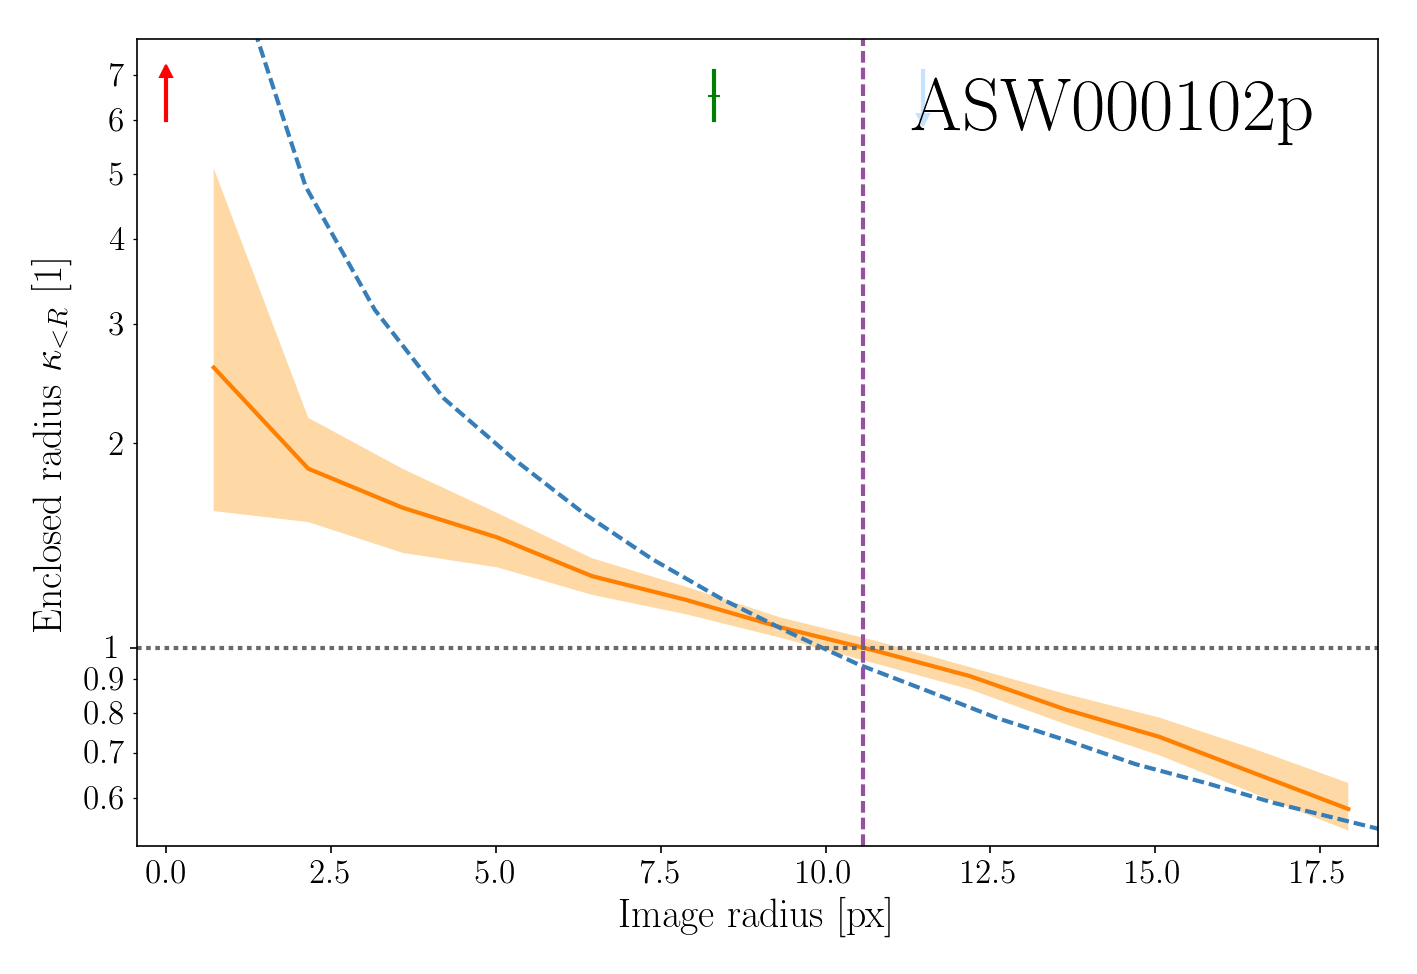
\includegraphics[width=.9\linewidth]{img/hires_comparison/ASW000102p_6941_11_hires_comparison}
  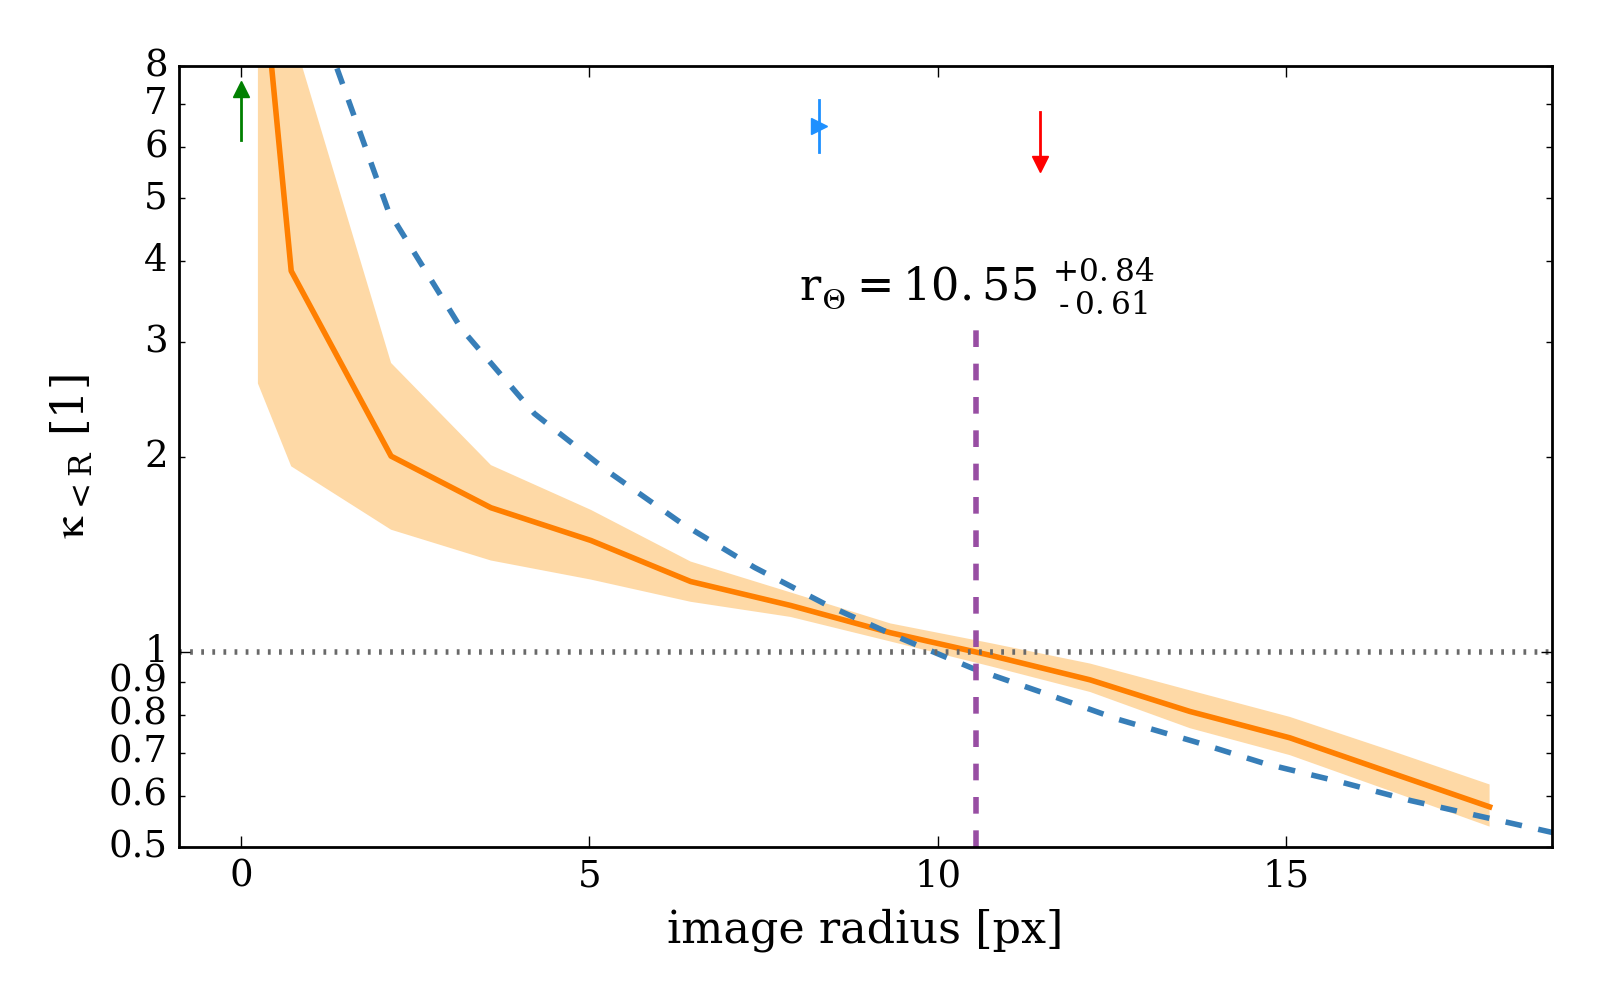
\includegraphics[width=.9\linewidth]{img/hires_comparison/ASW000102p_6941_13_hires_comparison}
  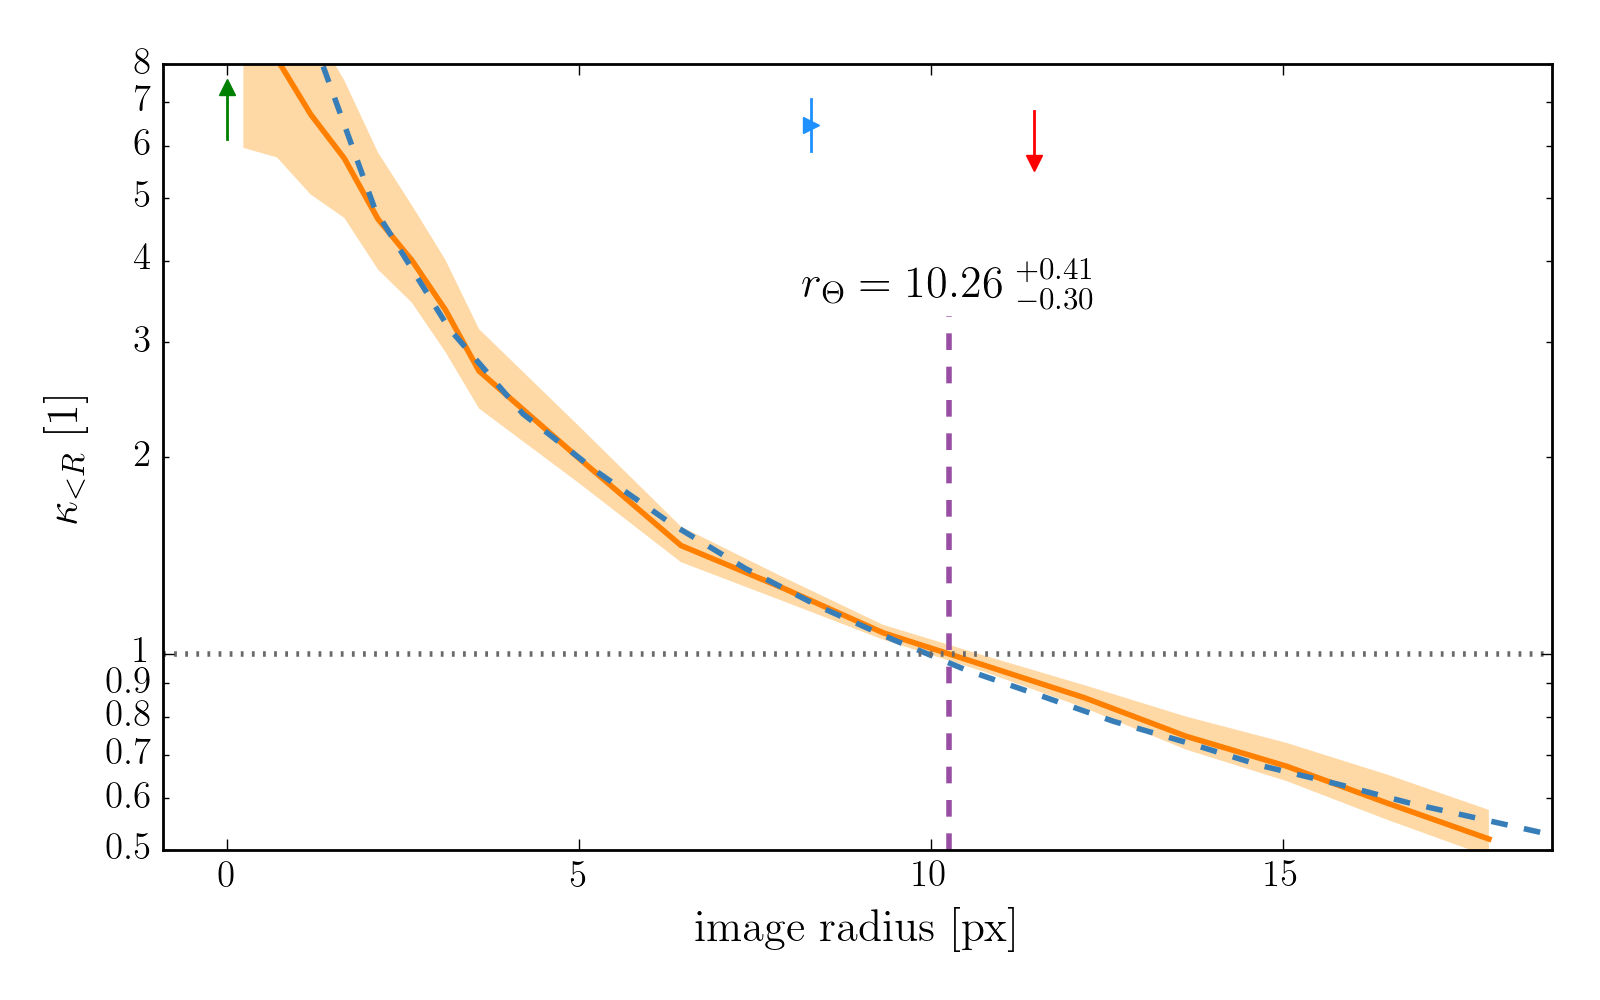
\includegraphics[width=.9\linewidth]{img/hires_comparison/ASW000102p_6941_33_hires_comparison}
  \caption{Model improvement resulting from using smaller mass tiles
    in the inner region of the mass model.  Shown here are the average
    enclosed $\kappa$ within a given projected radius, for three
    different reconstructions of a simulated lens (sim) from
    Space~Warps.  In each panel, the dashed blue curve is the correct
    answer.  The orange band represents the statistical ensemble from
    SpaghettiLens, the orange line being the ensemble mean.  Locations of
    images (maximum, saddle point, minimum) are marked with vertical
    arrows.  Crossing the horizontal $\kappa=1$ line is the effective
    Einstein radius \ER, and is so labelled. The upper panel is from
    K\"ung et al., (2015) (see Figure~3 of that paper).  The middle
    panel is the result when the innermost mass tile is replaced by 9
    smaller tiles.  The lower panel results from replacing each of the
    innermost 5 by 5 tiles each with 9 smaller tiles.}
  \label{fig:subsampling}
\end{figure}

\subsection{Sub-sampling of central region}\label{subsec:hires}

The models of simulated lenses in \cite{2015MNRAS.447.2170K} showed a
tendency to be too shallow.  Allowing smaller mass tiles in the
central region, thus allowing the mass profile to rise more steeply
near the centre, was suggested as a possible cure.

Figure~\figref{subsampling} shows an experiment with smaller mass
tiles in the inner region.  Replacing the very central mass tile with
9 smaller tiles allows for steeper central profiles.  Doing the same
for the 25 innermost mass tiles solves the problem completely, but
increases the number of mass tiles by 40\% and significantly increases
the computational time.
% 689 / 489 = 1.40899; in practice, runtime is more like x4 - x5!
% runtimes from logfiles: 87/22, 86/21, 85/16
The main modelling work in this paper was, however, done before the
experiments with smaller mass tiles was complete.  Some of the models
presented in this paper apply the intermediate option (corresponding
to the middle panel in Figure~\figref{subsampling}) while others use
the old system.  The results in this paper, however, mainly concern
the enclosed mass in the outer regions, so shallowness in the central
region should be inconsequential.

\subsection{Parameterisation of pixel models} \label{subsec:parameter}
In order to fit the set of pixelated models to a single parameterised model, a program was written that took a parameterised function and subtracted from it the mean and the principal components of the data, which were calculated using classical Principal Component Analysis.
This created the residuals function.
The number of components used in the analysis was varied, to test how this affected the output, and it was found that using 5 principle components tended to give a reasonable approximation.
A masking function was added which selected only the data points that fell inside the image of the lens, and the principal components were clipped in order to keep the values inside the region of the ensemble of models.
Any value higher than the clip was set to be the clip value.
This was chosen to be 2.5 as, assuming that the data follows a Gaussian error distribution, almost all the values for the variance should lie between 2 and 3 standard deviations from the mean.
Minimising the residuals function produces the set of parameters that fit the parameterised function to the original pixelated ensemble most closely.
A least squares fit was used to perform this minimisation.
The parameterised model function was obtained from the gravitational potential of an isothermal ellipsoid mass distribution \citep{2001astro.ph..2341K}.
This model is frequently used to describe gravitational lenses as it tends to fit well with observations.
The isothermal ellipsoid model outputs three useful parameters: the radius of the Einstein ring, the ellipticity of the model and the angle of the ellipticity from the vertical, giving the orientation of the galaxy.
By applying this model to simulated lenses for which the values of these parameters were already known, it was possible to gain an estimate of the projected accuracy of the results, before applying the model to the candidate lensing galaxies.

Preliminary results on recovery of Einstein radii are shown in
Figure~\ref{fig:parameter}. \todo{Einstein radii from parametric
  model-fitting.}

\begin{figure}
  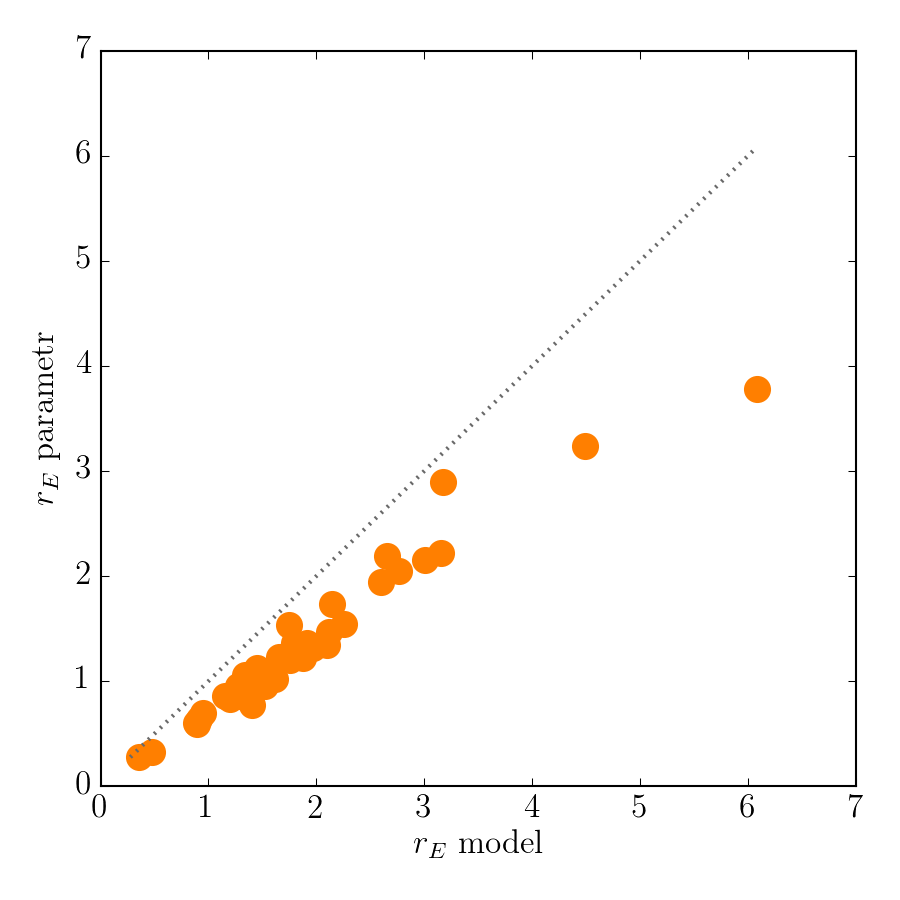
\includegraphics[width=\linewidth]{img/rE_comp/rE_comp.png}
  \caption{Comparison of Einstein radii. {\em To be extended.}}
  \label{fig:parameter}
\end{figure}


\section{TODO}
\listoftodos

% Don't change these lines
\bsp	% typesetting comment
\label{lastpage}
\end{document}



% \begin{figure}
%   \inclfign{SW05}{ASW0007k4r_N7LTELSYTM}
%   \caption{Model results for SW05 (J143454.4+522850).  See text in
%     Section~\ref{sec:examples} for details.}
%   \label{fig:SW05}
% \end{figure}
% 
% \begin{figure}
%   \inclfign{SW28}{ASW0007xrs_JHC3J2HYV7}
%   \caption{Model results for SW28 (J143055.9+572431).}
%   \label{fig:SW28}
% \end{figure}
% 
% \begin{figure}
%   \inclfign{SW02}{ASW000619d_011489}
%   \caption{Model results for SW02 (J140522.2+574333).}
%   \label{fig:SW02}
% \end{figure}
% 
% \begin{figure}
%   \inclfign{SW09}{ASW0002asp_5EKMWWVJHL}
%   \caption{Model results for SW09 (J020832.1-043315).}
%   \label{fig:SW09}
% \end{figure}
% 
% \begin{figure}
%   \inclfign{SW29}{ASW0008qsm_TOFS7JNGEK}
%   \caption{Model results for SW29 (J143838.1+572647).}
%   \label{fig:SW29}
% \end{figure}
% 
% \begin{figure}
%   \inclfig{SW42}{ASW00096rm_4Q3YCEWGLN}
%   \caption{Modelling results for SW42 (J221716.5+015826).}
%   \label{fig:SW42}
% \end{figure}
% 
% \begin{figure}
%   \inclfig{SW58}{ASW0007iwp_4XBJWT3COV}
%   \caption{Model results for SW58 (J143651.6+530705).}
%   \label{fig:SW58}
% \end{figure}
% 
% \begin{figure}
%   \inclfig{SW19}{ASW0001ld7_OS3CYAKLRT}
%   \caption{Model results for SW19 (J020642.0-095157).}
%   \label{fig:SW19}
% \end{figure}
% 
% 
% \begin{figure}
%   \inclfig{SW36}{ASW000096t_7IPP7LWVOF}
%   \caption{Model results for SW36 (J090248.4-010232).}
%   \label{fig:SW36}
% \end{figure}
% 
% \begin{figure}
%   \inclfig{SW57}{ASW0008pag_5SXGXQYY6V}
%   \caption{Model results for SW57 (J143631.5+571131).}
%   \label{fig:SW57}
% \end{figure}

